\cleardoublepage % memastikan bab baru dimulai di halaman ganjil (kanan)
\chapter{STUDI LITERATUR}
\label{chap:studi-literatur}
\section{\textit{Hypertext Transfer Protocol}}

\textit{Hypertext Transfer Protocol} (HTTP) adalah protokol level aplikasi \textit{stateless} untuk sistem informasi berbasis hiperteks terdistribusi dan kolaboratif \cite{fielding_http_2022}. Protokol ini banyak digunakan untuk komunikasi antar klien terutama pada aplikasi berbasis web dan API terbuka. Protokol ini penting karena menyetandarkan metode komunikasi antara \textit{client} dan \textit{server} sehingga memungkinkan kedua belah pihak melakukan komunikasi secara \textit{platform-independent}. 

Pada versi pertama HTTP yakni HTTP/1.0, HTTP bekerja dengan cara membangun koneksi TCP antara \textit{client} dan \textit{server} sebelum melakukan transfer data sebelum setiap melakukan \textit{request} terhadap \textit{server}. Setelah menerima \textit{response} dari \textit{server} koneksi TCP yang telah dibangun tadi ditutup. Cara kerja dari versi ini divisualisasikan pada Gambar \ref{fig:http10}

\begin{figure}[h]
\caption{Cara kerja HTTP/1.0}
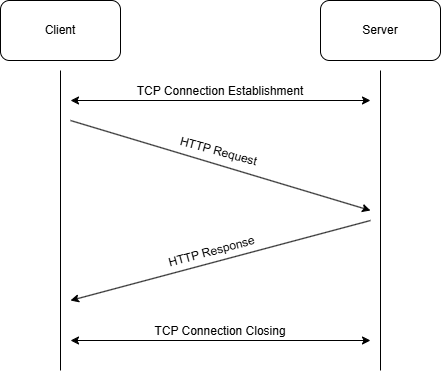
\includegraphics[scale=0.5]{images/HTTP10.png}
\label{fig:http10}
\end{figure}

Permasalahan dari HTTP/1.0 adalah koneksi TCP harus dibangun untuk setiap \textit{request} dan \textit{response} seperti yang divisualisasikan pada Gambar \ref{fig:http10_problem}. Selain itu, pada HTTP/1.0 setiap \textit{request} harus dikirimkan satu-per-satu sehingga setiap \textit{request} yang ingin dikirimkan harus menunggu \textit{response} dari \textit{request} sebelumnya. Hal ini tentu meningkatkan lama waktu interaksi antara \textit{client} dan \textit{server} serta membuang-buang \textit{bandwidth} yang tersedia. HTTP/1.1 dikembangkan untuk menangani masalah ini dengan menunda penutupan koneksi TCP hingga suatu kondisi yang dapat dikonfigurasi pada implementasi masing-masing web server (seringkali koneksi TCP baru akan ditutup jika tidak ada penggunaan koneksi dalam waktu \textit{timeout} yang dapat dikonfigurasi \cite{kurose_computer_2022}). HTTP/1.1 juga mendukung pengiriman banyak \textit{request} secara bersamaan, nantinya server akan menangani \textit{request-request} tersebut secara \textit{first-come-first-served} (FCFS). Cara kerja dari HTTP/1.1 divisualisasikan pada Gambar \ref{fig:http11}

\begin{figure}[h]
\caption{Skenario 2 \textit{request} dan \textit{response} pada HTTP/1.0}
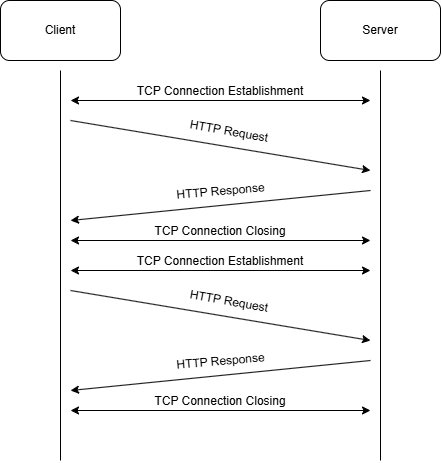
\includegraphics[scale=0.5]{images/HTTP10Problem.png}
\label{fig:http10_problem}
\end{figure}

\begin{figure}[ht]
\caption{Cara kerja HTTP/1.1}
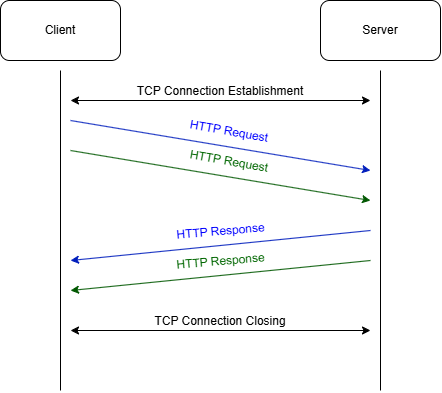
\includegraphics[scale=0.5]{images/HTTP11.png}
\label{fig:http11}
\end{figure}

Meskipun memiliki banyak keunggulan, pelayanan \textit{request}secara FCFS menimbulkan \textit{delay} pada suatu request jika terdapat \textit{request} yang datang sebelumnya yang membutuhkan \textit{response} besar. Masalah ini disebut sebagai \textit{Head of Line (HOL) blocking}. HTTP/2.0 dikembangkan dan mendukung \textit{multiplexing} yang memungkinkan banyak \textit{request} dikirimkan secara bersamaan serta mendukung \textit{field compression} untuk meningkatkan efisiensi pengiriman paket. HTTP/2.0 juga mendukung \textit{server push} yang memungkinkan server untuk mengirimkan \textit{response} yang dianggap akan dibutuhkan oleh \textit{client} untuk dikirimkan tanpa perlu menunggu adanya \textit{request} dari \textit{client} terlebih dahulu. Berbeda dengan HTTP/1.1, HTTP/2 tidak melayani \textit{request} secara FCFS sehingga dapat mengurangi masalah \textit{HOL Blocking}, meskipun begitu HTTP/2 tidak sepenuhnya menyelesaikan masalah HOL karena dari sisi TCP, permasalahan yang terjadi pada salah satu \textit{request}, dapat menghambat seluruh \textit{request} yang dikirimkan secara bersamaan tersebut.

HTTP/3 dikembangkan untuk mengatasi masalah ini. Pada HTTP/3, setiap pasangan \textit{request} dan \textit{response}, disebut sebagai \textit{stream}, bersifat independen sehingga permasalahan yang ada pada salah satu \textit{stream} tidak akan mengganggu \textit{stream} lainnya. Hal ini disebut sebagai \textit{stream-based multiplexing}. HTTP/3 juga menggunakan QUIC yang berjalan diatas UDP, sehingga memungkinkan proses inisialisasi koneksi yang lebih cepat dibanding HTTP versi sebelumnya yang masih berjalan diatas TCP. 

\begin{figure}[ht]
\caption{Perbandingan HTTP/2 \& HTTP/3}
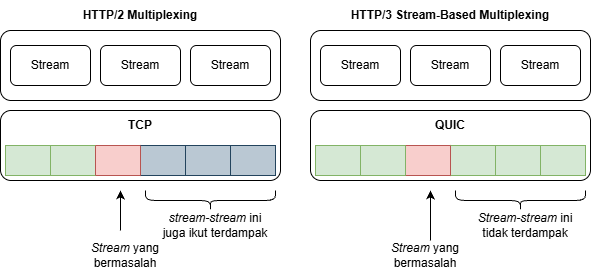
\includegraphics[scale=0.5]{images/HTTP2vHTTP3.png}
\label{fig:http2v3}
\end{figure}

\section{Penelitian Terkait}
\subsection{A}